\documentclass[11pt]{beamer}
\usetheme{Warsaw}
\usepackage[utf8]{inputenc}
\usepackage{amsmath}
\usepackage{amsfonts}
\usepackage{amssymb}
\usepackage{graphicx}

\graphicspath{{images/}}

%\begin{figure}[h!]
%\begin{center}
%\includegraphics[scale = 0.5]{exercise_3_11_a.png}
%\caption{SAS Output for $X^2$ and $G^2$ tests}
%\end{center}
%\end{figure}

\setbeamerfont{itemize/enumerate}{size=8pt}

\author{Collin Nolte}
\title[AMCS Seminar Talk]{Supervised Principal Components for Classification}
\setbeamercovered{transparent} 
\setbeamertemplate{navigation symbols}{} 
%\logo{} 
%\institute{} 
\subtitle{An Odyssey}
\date{September 21, 2018} 

\begin{document}

\begin{frame}
\titlepage
\end{frame}

\begin{frame}
\frametitle{Table of Contents}
\tableofcontents
\end{frame}

\section{Motivation}
%\begin{frame}
%\frametitle{Introduction}
%{
%\textbf{Setting:} 
%\begin{align*}
%&\text{Features: } &X \in \mathbb{R}^p \\
%&\text{Outcome: } &Y = \{ 0,1 \} \\
%&\text{Small Sample Size: } & n=20 \text{ to } 40 \\ 
%&\text{Training Data Set: } &S_{train} \\
%&\text{Classifier Based on Training Data Set: } & g(S_{train}, \cdot)
%\end{align*}
%
%\textbf{Goal:}  Estimate the true error:
%
%\begin{equation*}
%\epsilon_n = \epsilon (g(S_{train}, \cdot)) = E_F (|Y-g(S_{train}, X)|)
%\end{equation*}
%
%In practice, we will settle for estimating the expectation of the true error $E[ \epsilon_n]$.
%}
%\end{frame}


\begin{frame}
\frametitle{Similarity to Sparse PCA}
{
Sparse PCA can be thought of as penalized regression of loadings onto $X_{n \times p} = UDV^T$
\begin{itemize}
  \item $UD$ represent the (scaled) principal components
  \item $V^T$, the loadings of $X$, is orthonormal, where $VV^T = I$, and each column is associated with a feature in $X$
  \item Post multiplying each side by $V$, we get
  \begin{align*}
  XV = UD = P
  \end{align*}
  \item We then choose our loadings $\tilde{v}_i$ for each column of $p_i$ separately such that $\tilde{v}_i$ is subject to the constraints
\end{itemize}
\begin{align*}
\min_{V} \frac{1}{N} \sum_{i=1}^N L(p_i,  v_i^Tx_i) + \lambda[(1-\alpha)||v_i||_2^2 + \alpha ||v_i||_1]
\end{align*}
}
\end{frame}

\begin{frame}
\frametitle{Similarity II}
{
\begin{itemize}
	\item glmnet style regression works best, as traditional Lasso limits total features to $n$, due to $L_1$ penalty
	\item This will create a number of $0$ loadings, resulting in sparse principal component  matrix
	\item This construction is "unsupervised", in that the final selection of $\tilde{V}$
	\item Once $\tilde{V}$ has been determined, we can perform regression in the standard way, using our sparse principal components
	\begin{align*}
	Y = \beta_0 + \sum_{m=1}^M \beta_m\tilde{P}_m  + \epsilon 
	\end{align*}
\end{itemize}
}
\end{frame}

\section{Method}
\begin{frame}
\frametitle{Latent Model Assumption}
{
\begin{itemize}
\item We imagine a situation in which $Y$ is a linear function of some latent variable $U$, where
\begin{align*}
Y = \beta_0 + \sum_{m = 1}^M \beta_m U_m + \epsilon
\end{align*}
\item Further, suppose each feature of $X$, say, $X_j$, captures some portion of this latent feature, so that
\begin{align*}
X_j = a_{0j} + \sum_{m=1}^M \alpha_{1jm} U_m + \epsilon_j
\end{align*}
\item We reconsider sparse PCA, but seek to select those $X_j$ which best capture the latent variable $U$
\end{itemize}
}
\end{frame}


\begin{frame}
\frametitle{Method}
{
\begin{itemize}
\item Represent each $X_j$ as the linear combination of it's principal components $(UD)$, with coefficients $\alpha_{1jm} = V_{[j,m]}$
\item We now go about selecting loadings $V^*$, not so that we retain the structure of $X$, but so that we capture information related to our latent variable $U$
\item If $\textbf{s}$ represents the standardized regression coefficient measuring the univariate effect of each feature of $X$ on $Y$,
\begin{align*}
s_j = \frac{x_j^Ty}{||x_j||}
\end{align*}
we seek a collection of features $C_{\theta}$ such that $|s_j| > \theta$
\end{itemize}
}
\end{frame}



\section{Model Training and Results}
\begin{frame}
\frametitle{Dataset Summary}
{\small
\begin{itemize}
\item Our analysis consists of three independent datasets collected from the National Center for Biotechnology Information (NCBI)
\item  Common genes were selected amongst the three datasets, and 40 percent were removed at random for memory constraint issues (13325 total)
\item The two primary datasets contain gene expressions from heart (313) and liver (77) tissues, without outcomes being heart failure and Type II diabetes
\item The third dataset (24)  has outcomes related to both heart disease and diabetes, and is used as an additional out of sample measure of prediction performance
\end{itemize}
}
\end{frame}

\begin{frame}
\frametitle{Models Used}
{
For each dataset, the following models were built and considered in caret using 10 fold cross validation
\begin{itemize}
\item Supervised PCA with threshold $\theta$ as a tuning parameter (fit with glm and lda)
\item glmnet with $\alpha = 1/\epsilon$, and tuning parameter $\lambda$ (sparse PCA)
\item AdaBoost.M1 with parameters tree and tree depth
\item Partial least squares with number of components as tuning parameters
\end{itemize}
}
\end{frame}


\begin{frame}
\frametitle{Supervise PCA Performance - Heart}
\begin{columns}
\column{0.5\textwidth}

{\footnotesize
\begin{itemize}
\item Model 5 is AdaBoost
\item Model 4 is partial least squares
\item Model 3 is glmnet
\item Models 1 and 2 represent supervised PCA with glm and lda, respectively
\end{itemize}
}
\column{0.5\textwidth}
%
\begin{figure}
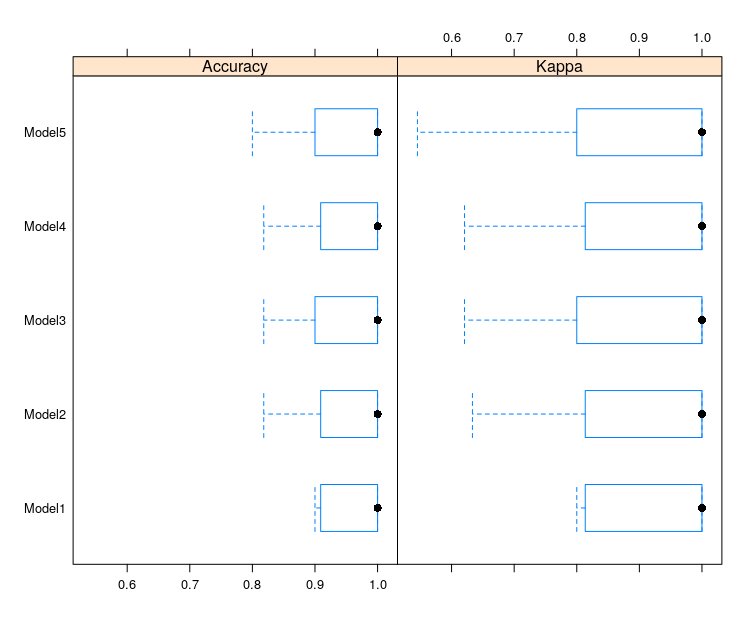
\includegraphics[scale = 0.25]{modelCompareHeart.png} \\
%\includegraphics[scale = 0.25]{box3.png} \\
%\includegraphics[scale = 0.15]{legend.png}
\end{figure}
\end{columns}
\end{frame}

\begin{frame}
\frametitle{Supervise PCA Performance - Liver}
\begin{columns}
\column{0.5\textwidth}

{\footnotesize
\begin{itemize}
\item Model 5 is AdaBoost
\item Model 4 is partial least squares
\item Model 3 is glmnet
\item Models 1 and 2 represent supervised PCA with glm and lda, respectively
\end{itemize}
}
\column{0.5\textwidth}
%
\begin{figure}
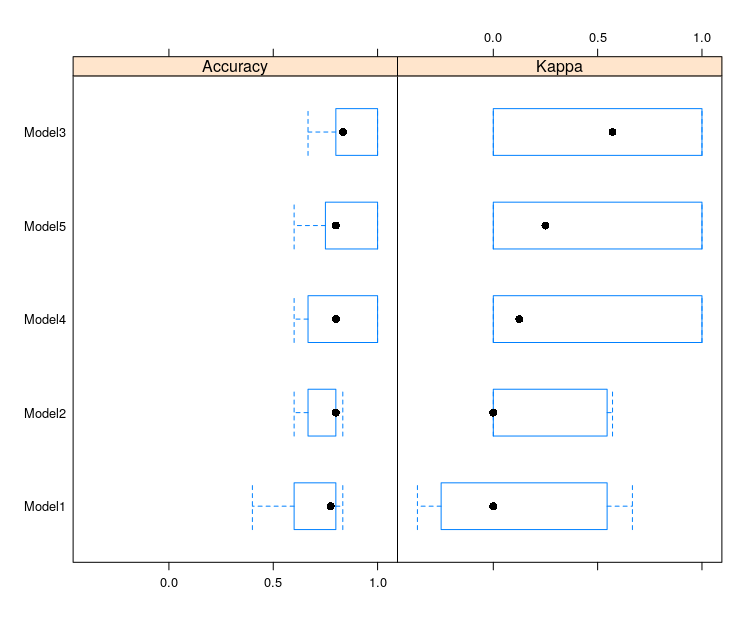
\includegraphics[scale = 0.25]{resampPlotLiver.png} 
\end{figure}
\end{columns}
\end{frame}



\section{Variable Importance}
\begin{frame}
\frametitle{Variable Importance Heart Data}
{

\begin{figure}
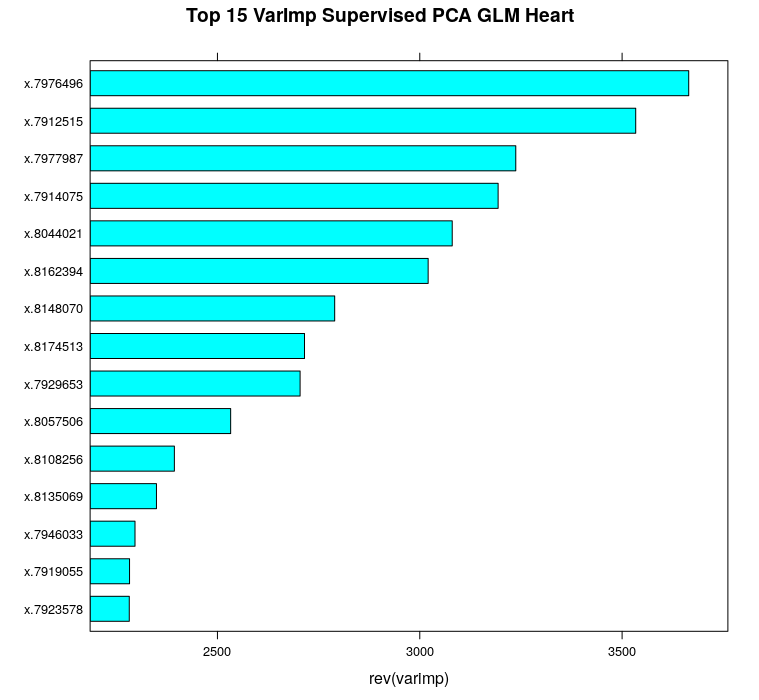
\includegraphics[scale=0.2]{heartVarImp_glm.png}
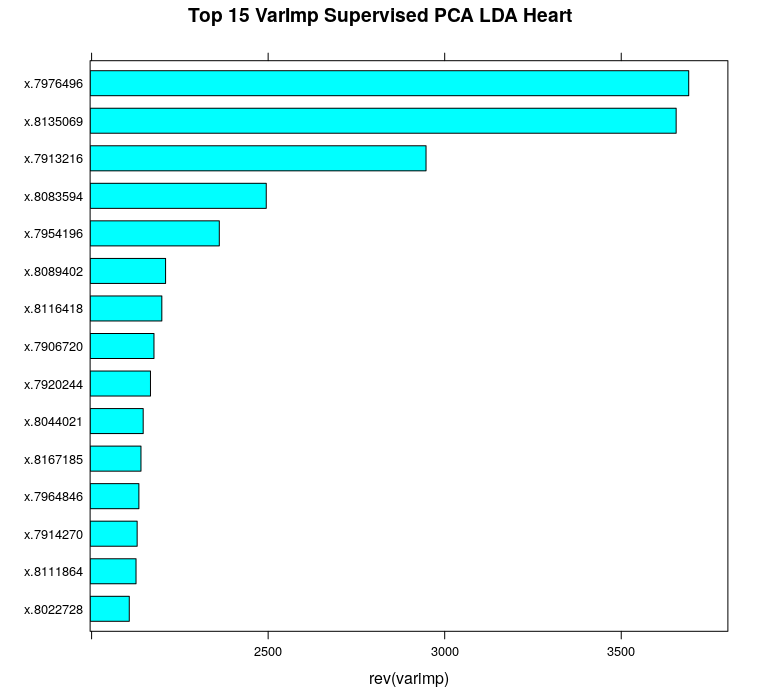
\includegraphics[scale=0.2]{heartVarImp_lda.png}
\end{figure}

\begin{itemize}
\item Define $varImp(x_j) = \sum_{i=1}^m <x_j, u_{\theta, i} >$
\item GLM retained 3155 out of 13325 genes, and LDA retained 1988 genes
\item GLM retained each of the 1988 retained in best LDA model
\end{itemize}
}
\end{frame}

\begin{frame}
\frametitle{Focus on Sparsity - Heart}
{
\begin{figure}
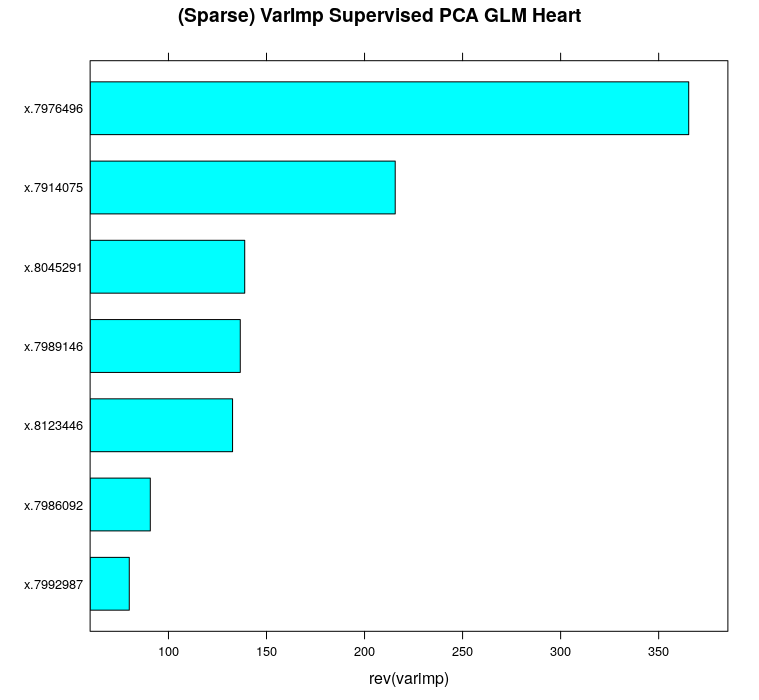
\includegraphics[scale=0.2]{heartVarImp_glmSparse.png}
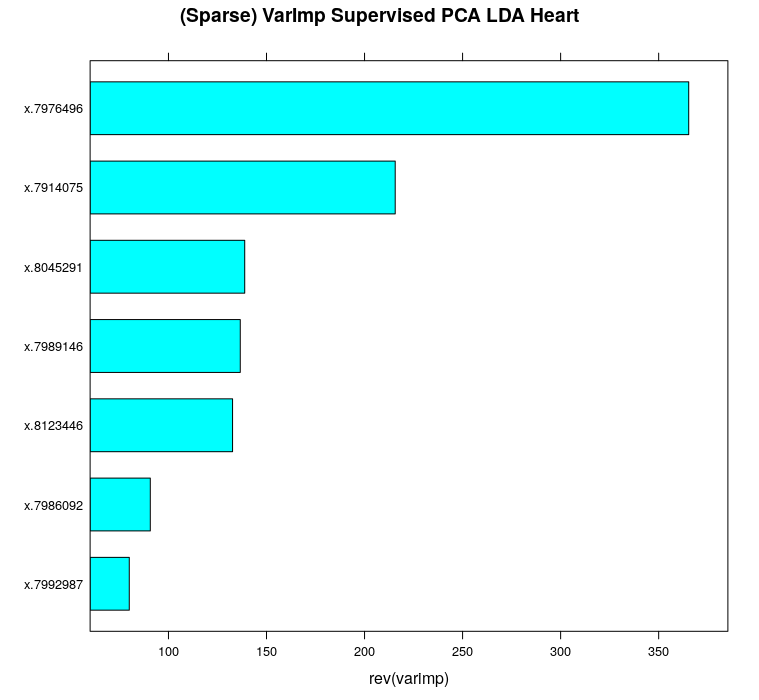
\includegraphics[scale=0.2]{heartVarImp_lda_Sparse.png}
\end{figure}

\begin{itemize}
\item In most sparse matrices, 7 genes are retained in each
\end{itemize}
}
\end{frame}


\begin{frame}
\frametitle{Variable Importance Liver Data}
{

\begin{figure}
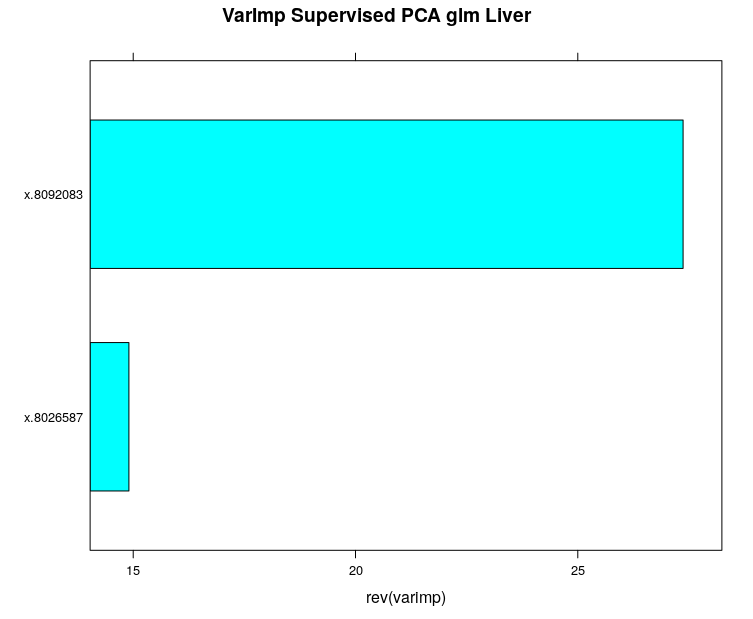
\includegraphics[scale=0.2]{liverVarImp_glm.png}
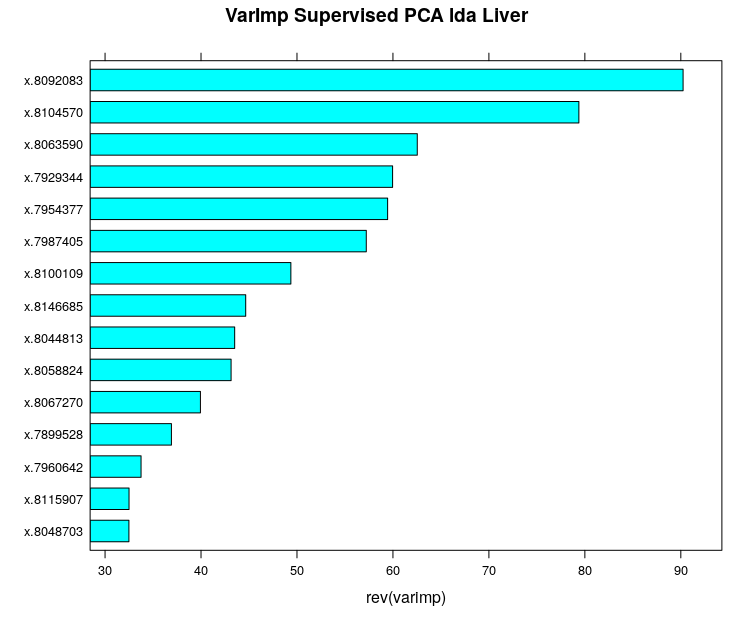
\includegraphics[scale=0.2]{liverVarImp_lda.png}
\end{figure}

\begin{itemize}
\item Define $varImp(x_j) = \sum_{i=1}^m <x_j, u_{\theta, i} >$
\item GLM retained 2 out of 13325 genes, and LDA retained 15 genes
\item LDA retained both genes from GLM
\end{itemize}
}
\end{frame}

\begin{frame}
\frametitle{Focus on Sparsity - Liver}
{
\begin{figure}
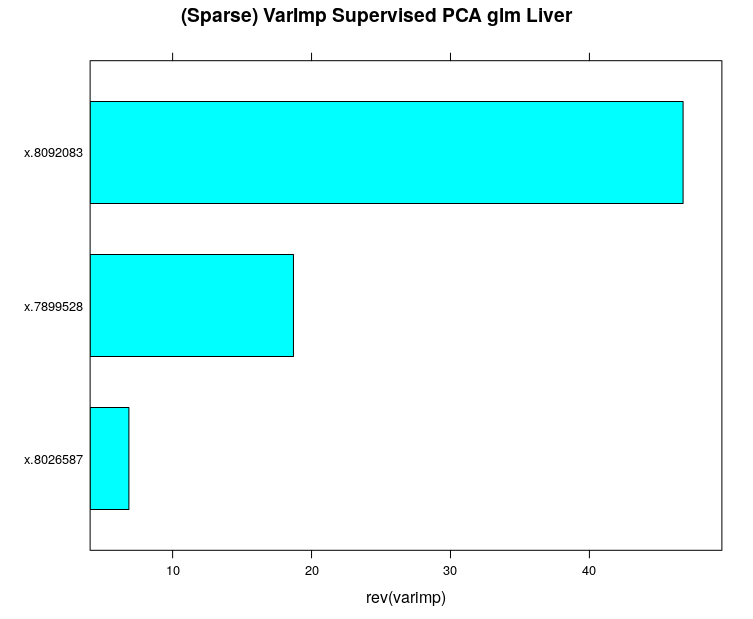
\includegraphics[scale=0.2]{liverVarImp_glmSparse.png}
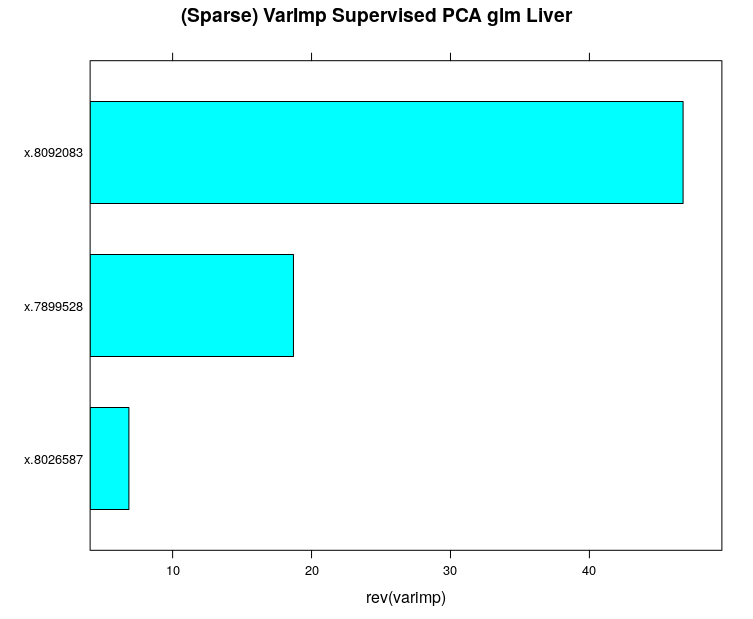
\includegraphics[scale=0.2]{liverVarImp_lda_Sparse.png}
\end{figure}

\begin{itemize}
\item In most sparse matrices, 7 genes are retained in each
\end{itemize}
}
\end{frame}






\begin{frame}
\frametitle{Final Model Summaries - Heart}
{
\begin{table}[ht]
\centering
\resizebox{\columnwidth}{!}{%
\begin{tabular}{rrrrr}
  \hline
 & GLM in-sample & GLM out-sample & LDA in-sample & LDA out-sample \\ 
  \hline
Accuracy & 0.932 & 0.942 & 0.942 & 0.916 \\ 
  Kappa & 0.862 & 0.779 & 0.881 & 0.779 \\ 
   \hline
\end{tabular}
}
\caption{Best fitting models from Sparse PCA (3155 and 1988 genes)}
\end{table} 

\begin{table}[ht]
\centering
\resizebox{\columnwidth}{!}{%
\begin{tabular}{rrrrr}
  \hline
 & GLM in-sample & GLM out-sample & LDA in-sample & LDA out-sample \\ 
  \hline
Accuracy & 0.952 & 0.916 & 0.942 & 1.00 \\ 
  Kappa & 0.902 & 0.780 & 0.881 & 1.00 \\ 
   \hline
\end{tabular}
}
\caption{Sparsest Models using Sparse PCA (7 genes)}
\end{table}
}
\end{frame}



\begin{frame}
\frametitle{Final Model Summaries - Liver}
{
\begin{table}[ht]
\centering
\resizebox{\columnwidth}{!}{%
\begin{tabular}{rrrrr}
  \hline
 & GLM in-sample & GLM out-sample & LDA in-sample & LDA out-sample \\ 
  \hline
Accuracy & 0.760 & 0.708 & 0.800 & 0.760 \\ 
  Kappa & 0.667 & 0.030 & 0.000 & 0.030 \\ 
   \hline
\end{tabular}
}
\caption{Best fitting models from Sparse PCA (2 and 15 genes)}
\end{table} 

\begin{table}[ht]
\centering
\resizebox{\columnwidth}{!}{%
\begin{tabular}{rrrrr}
  \hline
 & GLM in-sample & GLM out-sample & LDA in-sample & LDA out-sample \\ 
  \hline
Accuracy & 0.760 & 0.666 & 0.760 & 0.666 \\ 
  Kappa & 0.342 & 0.000 & 0.342 & 0.030 \\ 
   \hline
\end{tabular}
}
\caption{Sparsest Models using Sparse PCA (3 genes)}
\end{table}
}
\end{frame}

\begin{frame}
\frametitle{Final Summaries}
{
\begin{itemize}
\item By comparison, glmnet retained 17 and 26 genes in the heart and liver.

\end{itemize}
\begin{table}[ht]
\centering
\resizebox{\columnwidth}{!}{%
\begin{tabular}{rrrrr}
  \hline
 & glmnet Heart in-sample & glmnet Heart out-sample & glmnet Liver in-sample & glmnet Liver out-sample \\ 
  \hline
Accuracy & 0.966 & 1.00 & 0.920 & 0.292 \\ 
  Kappa & 0.931 & 1.00 & 0.781 & 0.000 \\ 
   \hline
\end{tabular}
}
\caption{glmnet in Heart and Liver (17 and 16 samples, respectively)}
\end{table}

}
\end{frame}


\section{Conclusion}
\begin{frame}
\frametitle{Conclusions}
{
\begin{itemize}
\item Supervised PCA achieves high sparsity in the loadings of $X$ while retaining structure of latent variable $U$
\item Performs better, relative to others, with larger sample sizes
\item Out of sample prediction is also superior in some cases
\item Remarkably, retains a set of genes entirely independent from those selected in glmnet.
\end{itemize}
}
\end{frame}


\begin{frame}
\frametitle{Sources}
\begin{itemize}\scriptsize
\item R Development Core Team (2008). R: A language and environment for
  statistical computing. R Foundation for Statistical Computing,
  Vienna, Austria. ISBN 3-900051-07-0, URL http://www.R-project.org.
\item Max Kuhn. Contributions from Jed Wing, Steve Weston, Andre Williams,
  Chris Keefer, Allan Engelhardt, Tony Cooper, Zachary Mayer, Brenton
  Kenkel, the R Core Team, Michael Benesty, Reynald Lescarbeau, Andrew
  Ziem, Luca Scrucca, Yuan Tang, Can Candan and Tyler Hunt. (2018).
  caret: Classification and Regression Training. R package version
  6.0-79. https://CRAN.R-project.org/package=caret
 \item Max Kuhn and Hadley Wickham (2018). recipes: Preprocessing Tools to
  Create Design Matrices. R package version 0.1.2.
  https://CRAN.R-project.org/package=recipes

\item BIOS 6720 course notes
\item   Matt Dowle and Arun Srinivasan (2017). data.table: Extension of
  `data.frame`. R package version 1.10.4-3.
  https://CRAN.R-project.org/package=data.table
\end{itemize}
\end{frame}

\begin{frame}
\frametitle{Sources cont.}
\begin{itemize}\scriptsize
\item   Hadley Wickham (2018). stringr: Simple, Consistent Wrappers for
  Common String Operations. R package version 1.3.0.
  https://CRAN.R-project.org/package=stringr
\item   Orchestrating high-throughput genomic analysis with Bioconductor. W.
  Huber, V.J. Carey, R. Gentleman, ..., M. Morgan Nature Methods,
  2015:12, 115.
\item   Davis, S. and Meltzer, P. S. GEOquery: a bridge between the Gene
  Expression Omnibus (GEO) and BioConductor. Bioinformatics, 2007, 14,
  1846-1847
\item "Elements of Statistical Learning", Trevor Hastie, Robert Tibshirani, Jerome Friedman.
\item Bair, Eric, et al. “Prediction by Supervised Principal Components.” Journal of the American Statistical Association, vol. 101, no. 473, 2006, pp. 119–137., doi:10.1198/016214505000000628. 
\end{itemize}
\end{frame}


\end{document}
